%Version 3.1 December 2024
% ESE 5760 Final Project — SRAM PVT Analysis
%
%%%%%%%%%%%%%%%%%%%%%%%%%%%%%%%%%%%%%%%%%%%%%%%%%%%%%%%%%%%%%%%%%%%%%%
%%                                                                 %%
%% Please do not use \input{...} to include other tex files.       %%
%% Submit your LaTeX manuscript as one .tex document.              %%
%%                                                                 %%
%% All additional figures and files should be attached             %%
%% separately and not embedded in the \TeX\ document itself.       %%
%%                                                                 %%
%%%%%%%%%%%%%%%%%%%%%%%%%%%%%%%%%%%%%%%%%%%%%%%%%%%%%%%%%%%%%%%%%%%%%

\documentclass[pdflatex,sn-mathphys-num,iicol]{sn-jnl}% 2-column Math/Phys numbered style

%%%% Standard Packages
\usepackage{graphicx}%
\usepackage{multirow}%
\usepackage{amsmath,amssymb,amsfonts}%
\usepackage{amsthm}%
\usepackage{mathrsfs}%
\usepackage[title]{appendix}%
\usepackage{xcolor}%
\usepackage{textcomp}%
\usepackage{manyfoot}%
\usepackage{booktabs}%
\usepackage{algorithm}%
\usepackage{algorithmicx}%
\usepackage{algpseudocode}%
\usepackage{listings}%

\theoremstyle{thmstyleone}%
\newtheorem{theorem}{Theorem}%
\newtheorem{proposition}[theorem]{Proposition}%

\theoremstyle{thmstyletwo}%
\newtheorem{example}{Example}%
\newtheorem{remark}{Remark}%

\theoremstyle{thmstylethree}%
\newtheorem{definition}{Definition}%

\raggedbottom

\begin{document}

\title[SRAM PVT Analysis]{Process--Voltage--Temperature Analysis of a 6T SRAM Bitcell and a 128$\times$128 Array Macro}

\author*[1]{\fnm{Krishna Karthikeya} \sur{Chemudupati}}\email{krishkc@seas.upenn.edu}

\author[1]{\fnm{Taarana} \sur{Jammula}}\email{taaranaj@seas.upenn.edu}

\author[1]{\fnm{Adithya} \sur{Selvakumar}}\email{adisel@seas.upenn.edu}

\affil*[1]{\orgdiv{Department of Electrical and Systems Engineering}, \orgname{University of Pennsylvania}, \orgaddress{\city{Philadelphia}, \state{PA}, \country{USA}}}

\abstract{We characterize a 6T SRAM bitcell across three process--voltage corners (FF~1.2~V, TT~1.0~V, SS~1.0~V, with SS~0.8~V where the metric is defined) and bridge the cell-level evidence to a 128$\times$128, 8-bit, 16:1 column-multiplexed macro modeled in NVSim. Stability and writability are extracted from butterfly curves (largest-square limiting eye for read and hold SNM, diagonal-corner write noise margin) and from a transient pulse-window read-disturb metric. We compare the baseline cell against three optimizations: a high-$V_t$ access-transistor variant, a negative-bitline write assist, and a wordline-underdrive read assist. The optimized cells trade margin for power or speed in expected ways: high-$V_t$ reduces TT hold-window energy by 13.9\,\% at the cost of a 10.2\,\% read-SNM penalty; negative-bitline cuts TT write delay by 54.5\,\%; and wordline-underdrive raises TT read SNM by 39.9\,\% while suppressing read disturb by 57.3\,\%. Every macro number is labeled by its evidence type (\emph{Estimated by NVSim}, \emph{Measured in Cadence}, or \emph{Derived proxy}) so that NVSim outputs are never silently mixed with Cadence-derived bridges.}

\keywords{SRAM, 6T bitcell, PVT, SNM, write noise margin, NVSim, high-$V_t$, negative bitline, wordline underdrive}

\maketitle

%-----------------------------------------------------------------------
\section{Introduction}\label{sec:intro}

Static random-access memory (SRAM) sets the area, energy, and access-time floor of most modern systems-on-chip, and its margins are the part of the chip most exposed to process--voltage--temperature (PVT) variation. A six-transistor (6T) bitcell that holds reliably under one corner can lose read or write margin at another, and assist circuits added to recover that margin almost always trade off against either dynamic energy, leakage, or speed.

This work quantifies those trade-offs. We start from a single 6T bitcell, characterize its hold static noise margin (SNM), read SNM, and write noise margin (WNM) across the corners that matter, and then evaluate three commonly proposed optimizations against the same baseline:

\begin{enumerate}
    \item \textbf{High-$V_t$} access transistors, intended to reduce hold-window leakage at the cost of read-SNM.
    \item \textbf{Negative-bitline} write assist, intended to accelerate the write transition.
    \item \textbf{Wordline-underdrive} read assist, intended to recover read SNM and suppress read disturb.
\end{enumerate}

The cell-level evidence is then bridged into a 128$\times$128, 8-bit, 16:1 column-multiplexed macro modeled in NVSim. Because NVSim does not natively model the three optimizations, we keep every macro-level number labeled with its evidence type --- \emph{Estimated by NVSim}, \emph{Measured in Cadence}, or \emph{Derived proxy} --- so that simulator outputs are never silently mixed with Cadence-derived bridges.

%-----------------------------------------------------------------------
\section{Methodology}\label{sec:methodology}

\subsection{Bitcell SNM and WNM extraction}\label{sec:methodology-bitcell}

Hold SNM and read SNM are extracted from the standard butterfly DC sweeps of the storage node $V_Q$ versus the complementary node $V_{\overline{Q}}$. We use the largest-square limiting-eye fit: the SNM is the side length of the largest square that fits inside the smaller of the two eyes formed by the inverter and access-transistor characteristics. This is the conservative choice when the two lobes are asymmetric and is the convention used throughout the figures in Section~\ref{sec:baseline-bitcell}.

Write noise margin uses the diagonal-corner $V_1=V_2$ convention: WNM is the side length of the largest square anchored on the diagonal that fits between the read and write curves of the cell during a write. The same convention is used uniformly across the WNM butterfly figures, so the reported numbers are directly comparable across corners and across optimizations.

All bitcell metrics in this report are labeled \emph{Measured in Cadence}.

\subsection{Wordline-underdrive read disturb}\label{sec:methodology-readdisturb}

The wordline-underdrive read-disturb value is a transient pulse-window metric, not a DC quantity. It is the maximum disturbance of the storage node opposite to the access path, measured on $\overline{Q}$ during the read pulse window of the transient bench. This metric captures the dynamic node bounce that is the actual failure mechanism a wordline-underdrive assist is designed to suppress, and it is reported alongside the static read-SNM gain to avoid claiming a benefit that exists only in DC.

\subsection{Cadence-to-NVSim bridge}\label{sec:methodology-bridge}

The macro evaluation in Sections~\ref{sec:baseline-macro} and \ref{sec:bridged-macro} is anchored on a single direct NVSim run for the 128$\times$128, 8-bit, 16:1 baseline organization. From that anchor we apply optimization-specific changes to exactly the columns where the Cadence evidence justifies a change, and leave the rest at the NVSim baseline. Every row of the bridge carries one of three labels:

\begin{itemize}
    \item \emph{Estimated by NVSim} --- copied directly from the NVSim baseline run.
    \item \emph{Measured in Cadence} --- comes from the bitcell simulations and is included only as supporting evidence, not as a macro number.
    \item \emph{Derived proxy} --- a baseline NVSim number scaled by a Cadence-measured ratio at TT nominal, used only when there is no NVSim knob for the optimization in question.
\end{itemize}

The TT-nominal corner is the bridge anchor; corner robustness is left to the bitcell section. Concretely, only two macro columns receive a derived proxy in this report: the High-$V_t$ leakage power (scaled by the TT hold-window energy ratio) and the Negative-BL write latency (scaled by the TT write-delay ratio). Wordline-underdrive does not change any macro column because the assist's defended benefit is cell-level stability, not a macro timing or energy shift; we therefore present it in the bitcell results section only.

%-----------------------------------------------------------------------
\section{Baseline bitcell stability and writability}\label{sec:baseline-bitcell}

Hold SNM is comfortable at all three voltage--corner combinations (422--461\,mV), confirming that the cell holds robustly without assist. Read SNM is the smallest of the three margins (212--224\,mV) and sets the read-side reliability floor. WNM at TT nominal is 362\,mV; the SS~1.0\,V corner is the worst case at 259\,mV, which motivates the negative-bitline write assist evaluated in Section~\ref{sec:opt-negbl}. Per-corner butterfly overlays for hold SNM, read SNM, and WNM are reproduced in Appendix~\ref{secA:bitcell-overlays}.

%-----------------------------------------------------------------------
\section{Optimization studies}\label{sec:optimizations}

\subsection{High-$V_t$ access transistors}\label{sec:opt-highvt}

Raising the access-transistor threshold voltage cuts subthreshold leakage during the hold window, but it also weakens the access path and reduces read-SNM because the storage node is pulled less stiffly during a read. Figures~\ref{fig:highvt-energy} and \ref{fig:highvt-readsnm} report the two sides of this trade-off across corners.

\begin{figure}[t]
\centering
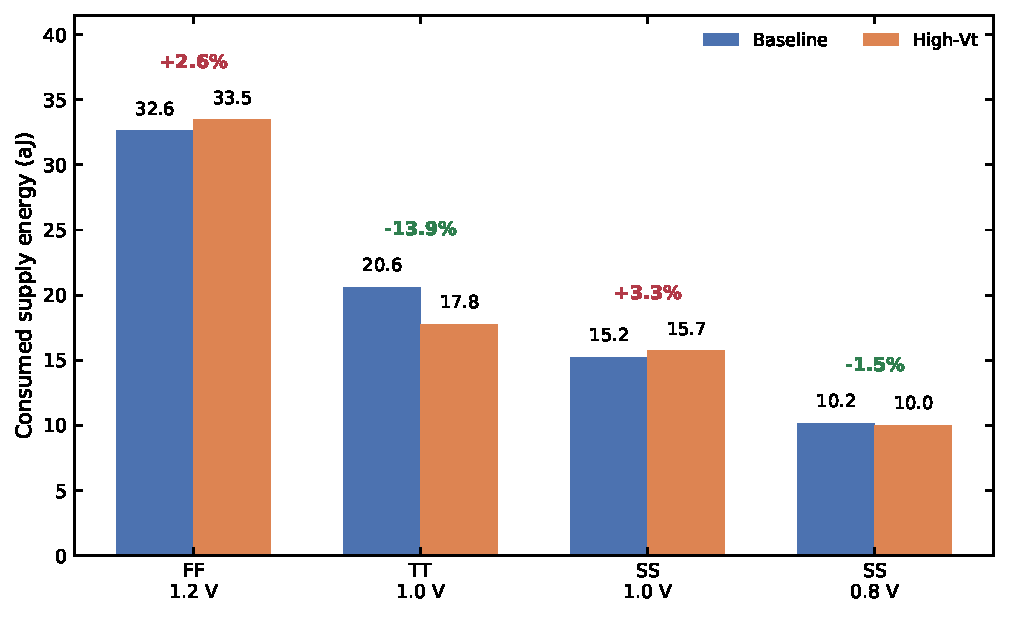
\includegraphics[width=\columnwidth]{figures/high_vt_hold_leakage_energy_by_corner.pdf}
\caption{Per-corner hold-window supply energy (6--9\,ns integration window) for the baseline cell versus the high-$V_t$ variant. TT~1.0\,V improves by 13.9\,\%; FF~1.2\,V regresses slightly because at the FF corner the leakage path is dominated by gate leakage that is not improved by raising $V_t$.}\label{fig:highvt-energy}
\end{figure}

\begin{figure}[t]
\centering
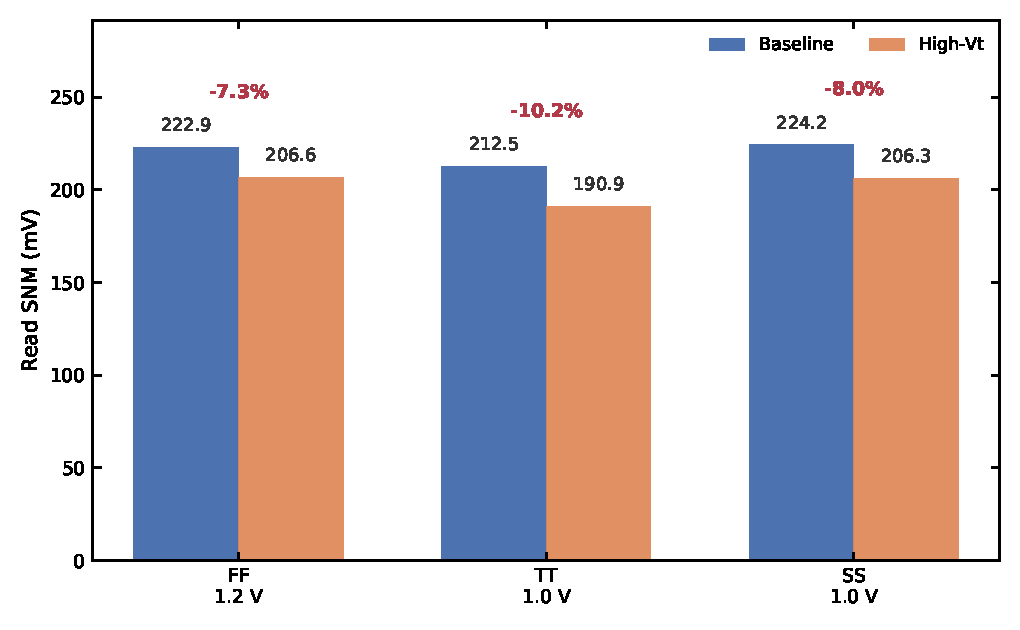
\includegraphics[width=\columnwidth]{figures/high_vt_read_snm_by_corner.pdf}
\caption{Per-corner read SNM for the baseline cell versus the high-$V_t$ variant, styled to pair visually with Figure~\ref{fig:highvt-energy}. SS~0.8\,V is intentionally absent because the baseline cell does not have a valid read butterfly at that supply without a wordline-underdrive assist; the limiting-eye SNM is therefore undefined.}\label{fig:highvt-readsnm}
\end{figure}

The TT-corner numbers summarize the trade-off cleanly: hold-window supply energy drops from 20.6\,aJ to 17.8\,aJ (-13.9\,\%), while read SNM drops from 212\,mV to 191\,mV (-10.2\,\%). Hold SNM degrades by less than 4\,\% at TT and by less than 3\,\% at SS~1.0\,V. The optimization is consistent with its intent at the typical and slow corners; the FF corner energy regression flags that high-$V_t$ is not a universal leakage win and motivates corner-aware deployment. Per-corner hold-SNM and read-SNM butterfly overlays are reproduced in Appendix~\ref{secA:bitcell-overlays}.

\subsection{Negative-bitline write assist}\label{sec:opt-negbl}

Driving the bitline below ground during the write strengthens the access transistor's pull-down ability and accelerates the storage-node flip. Figure~\ref{fig:negbl-writedelay} reports the WL-to-Q write delay for the assisted cell versus the baseline across all four corners.

\begin{figure}[t]
\centering
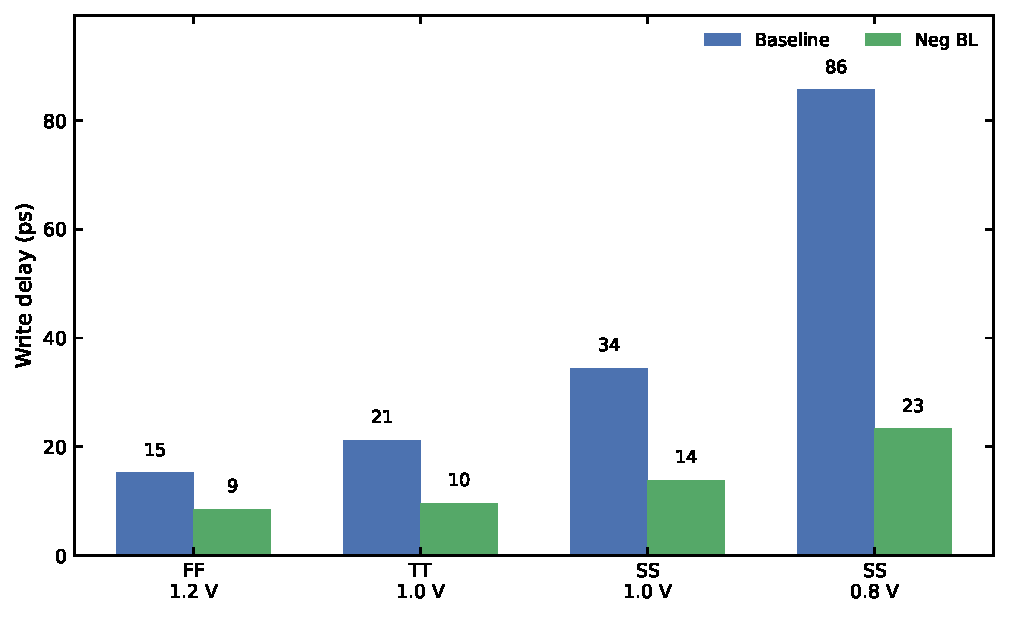
\includegraphics[width=\columnwidth]{figures/negative_bitline_write_delay_by_corner.pdf}
\caption{Per-corner WL-to-Q write delay for the baseline cell versus the negative-bitline assist. TT improves by 54.5\,\%; SS~0.8\,V improves by 72.8\,\%, the largest gain because that corner is the slowest baseline.}\label{fig:negbl-writedelay}
\end{figure}

The benefit grows monotonically as the corner slows, which is exactly the corner profile a write assist is supposed to have. The write-delay improvement at SS~0.8\,V (-72.8\,\%, from 85.6\,ps to 23.3\,ps) is the largest single-knob improvement reported in this work. The full per-corner waveform grid is reproduced in Appendix~\ref{secB:negbl-waveforms}.

\subsection{Wordline-underdrive read assist}\label{sec:opt-wlud}

Underdriving the wordline during a read keeps the access transistors weaker than the cross-coupled pull-down devices, which raises read SNM and suppresses the dynamic disturbance of the storage node. Figures~\ref{fig:wlud-readsnm} and \ref{fig:wlud-readdisturb} report the static and transient sides of this assist.

\begin{figure}[t]
\centering
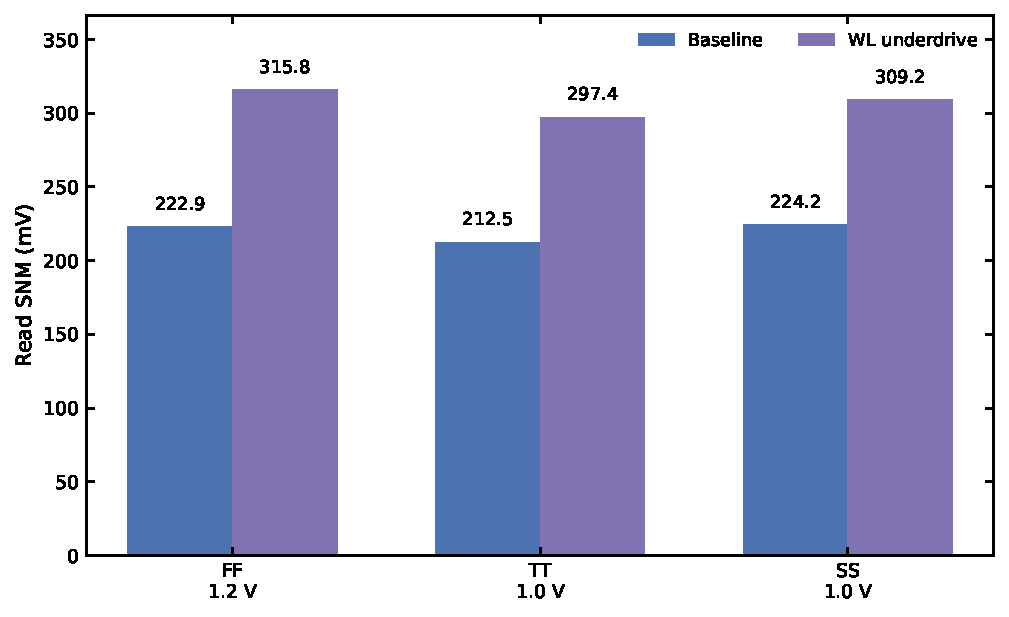
\includegraphics[width=\columnwidth]{figures/wordline_underdrive_read_snm_comparison.pdf}
\caption{Per-corner read SNM for the baseline cell versus the wordline-underdrive assist. TT improves by 39.9\,\% (212\,mV to 297\,mV); FF and SS~1.0\,V improve by similar margins.}\label{fig:wlud-readsnm}
\end{figure}

\begin{figure}[t]
\centering
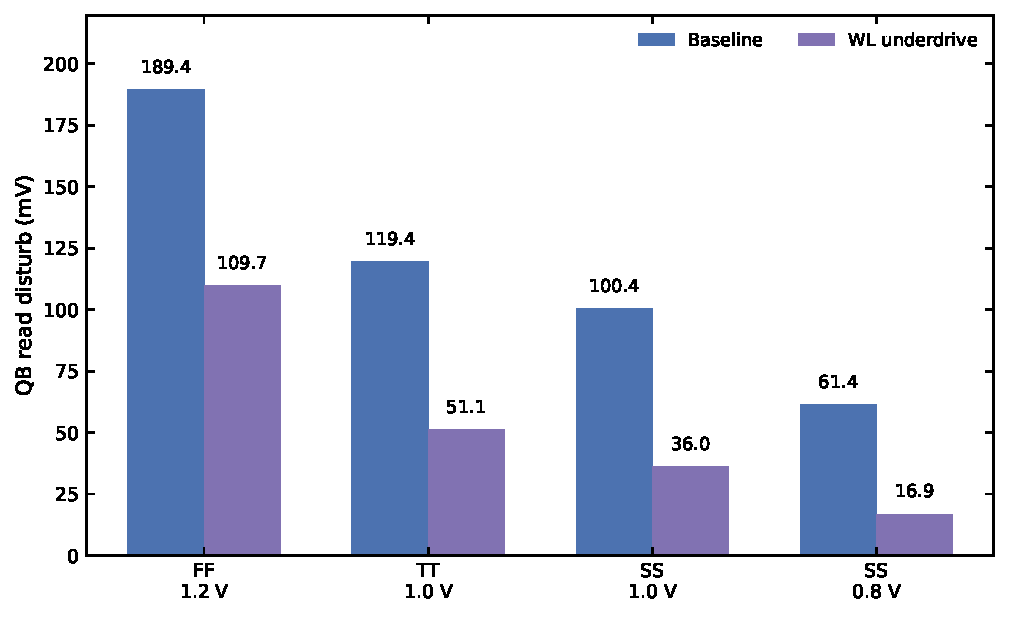
\includegraphics[width=\columnwidth]{figures/wordline_underdrive_read_disturb_comparison.pdf}
\caption{Per-corner pulse-window transient read-disturb metric (Section~\ref{sec:methodology-readdisturb}) for the baseline cell versus the wordline-underdrive assist. TT read disturb drops by 57.3\,\%; SS~0.8\,V drops by 72.5\,\%.}\label{fig:wlud-readdisturb}
\end{figure}

The static and transient evidence agree, which is the relevant cross-check: a read-SNM gain that did not show up in the transient read-disturb window would not be a real benefit. Both metrics improve at every corner, with the largest gains at the slowest, lowest-supply corner (SS~0.8\,V). The all-corner read-SNM butterfly overlay is reproduced in Appendix~\ref{secA:bitcell-overlays}.

%-----------------------------------------------------------------------
\section{Baseline NVSim macro}\label{sec:baseline-macro}

Table~\ref{tab:nvsim-baseline-macro} reports the direct NVSim baseline for the 128$\times$128, 8-bit, 16:1 organization. The full read-access latency budget breaks down as in Figure~\ref{fig:nvsim-latency-breakdown}.

\begin{table}[t]
\caption{Baseline NVSim macro summary at the locked organization (128$\times$128, 8-bit, 16:1). All rows are \emph{Estimated by NVSim}.}\label{tab:nvsim-baseline-macro}
\begin{tabular}{@{}lr@{}}
\toprule
\textbf{Baseline macro quantity} & \textbf{Value} \\
\midrule
Capacity & 2048 B \\
Physical array & 128 $\times$ 128 \\
Word width & 8 bits \\
Column selection & 16:1 \\
Area & 0.006197 mm$^2$ \\
Read latency & 0.8821 ns \\
Write latency & 0.8821 ns \\
Read energy & 1.3540 pJ \\
Write energy & 0.3210 pJ \\
Leakage & 0.4854 $\mu$W \\
\bottomrule
\end{tabular}
\end{table}

\begin{figure}[t]
\centering
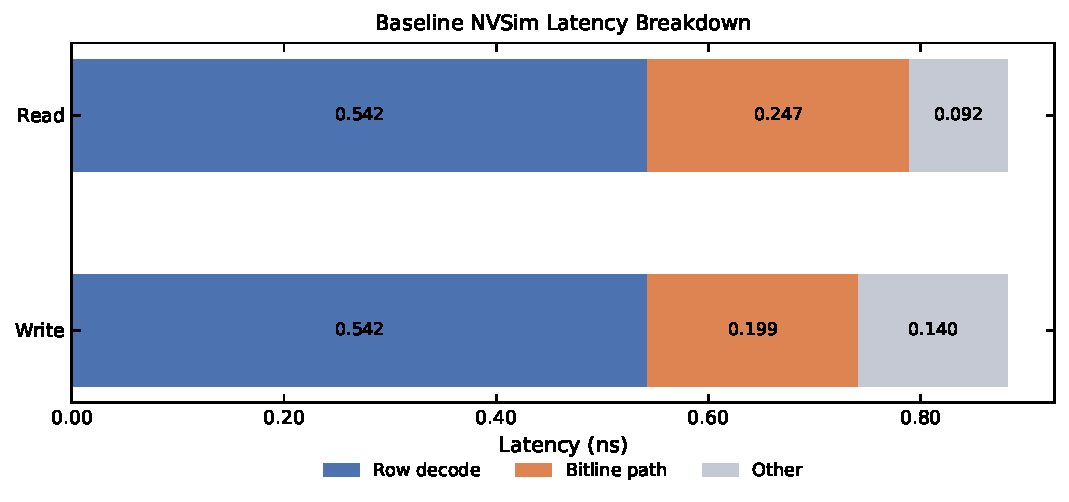
\includegraphics[width=\columnwidth]{figures/baseline_nvsim_latency_breakdown.pdf}
\caption{Latency budget for the baseline macro. Row decode (predecoder + row decoder) dominates both reads and writes at $\sim$61\,\% of total latency; the bitline path accounts for $\sim$28\,\% of read latency and $\sim$23\,\% of write latency.}\label{fig:nvsim-latency-breakdown}
\end{figure}

The breakdown makes clear that the row-decode path is where most of the macro's latency lives, and it is unaffected by any of the three bitcell optimizations evaluated in this report. That observation constrains which macro columns can plausibly move under each optimization.

%-----------------------------------------------------------------------
\section{Bridged optimization results}\label{sec:bridged-macro}

Per the bridge methodology of Section~\ref{sec:methodology-bridge}, only two macro columns move under the optimizations evaluated here: the high-$V_t$ leakage power and the negative-bitline write latency. Both are derived proxies anchored on the TT Cadence ratios; all other macro columns are reused from the NVSim baseline.

\subsection{High-$V_t$ macro leakage}\label{sec:bridged-highvt}

\begin{figure}[t]
\centering
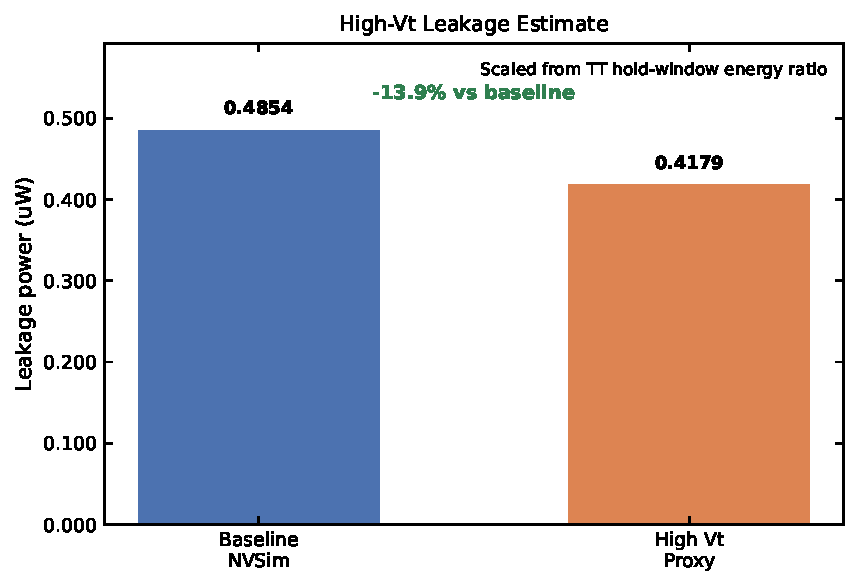
\includegraphics[width=\columnwidth]{figures/high_vt_leakage_proxy.pdf}
\caption{High-$V_t$ macro leakage power as a derived proxy: the baseline NVSim leakage (0.4854\,$\mu$W) scaled by the TT hold-window energy ratio (0.8610) gives 0.4179\,$\mu$W (-13.9\,\%). Area, latency, and dynamic energy stay at the NVSim baseline.}\label{fig:highvt-leakage-proxy}
\end{figure}

\subsection{Negative-BL macro write latency}\label{sec:bridged-negbl}

\begin{figure}[t]
\centering
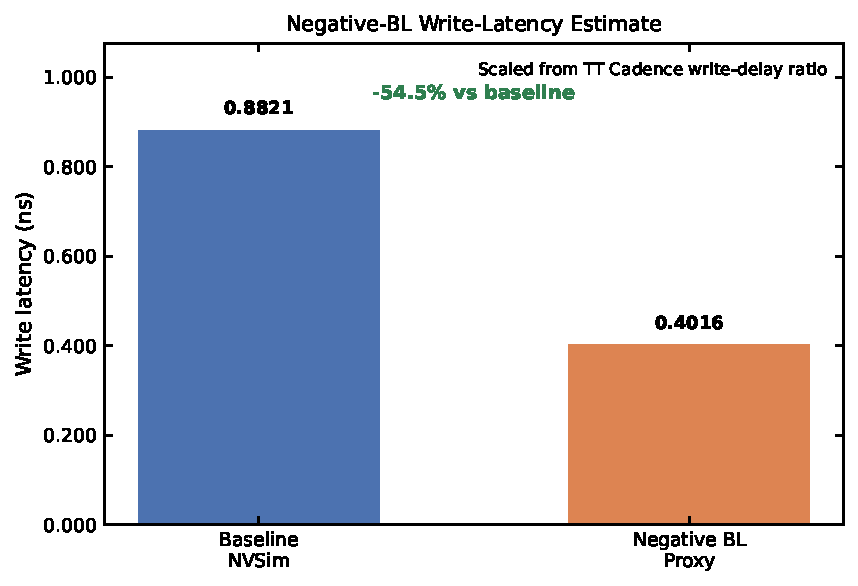
\includegraphics[width=\columnwidth]{figures/negative_bl_write_latency_proxy.pdf}
\caption{Negative-BL macro write latency as a derived proxy: the baseline NVSim write latency (0.8821\,ns) scaled by the TT Cadence write-delay ratio (0.4553) gives 0.4016\,ns (-54.5\,\%). Read latency, energy, and leakage stay at the NVSim baseline.}\label{fig:negbl-writelatency-proxy}
\end{figure}

\subsection{Why wordline-underdrive does not move a macro column}\label{sec:bridged-wlud}

The wordline-underdrive assist is real and well-supported by the cell-level evidence in Section~\ref{sec:opt-wlud}, but its benefit is read-SNM and read-disturb suppression, not a macro timing or energy shift that the bridge can defend. Forcing a derived-proxy column onto NVSim's macro row would therefore overclaim. The assist is presented in the bitcell results section and intentionally omitted from this section.

%-----------------------------------------------------------------------
\section{Cadence verification}\label{sec:cadence-verification}

Cadence verification of the 128$\times$128 macro at the schematic level is shown in Figures~\ref{fig:cadence-array}--\ref{fig:cadence-waveforms}. The screenshots confirm that the baseline organization assumed by NVSim (128 rows, 128 physical columns, 8-bit words, 16:1 column multiplexing) is the same organization reflected in the schematic and that the baseline access waveforms behave as intended.

\begin{figure}[t]
\centering
\fbox{\rule{0pt}{0.32\textheight}\rule{0.86\columnwidth}{0pt}}
\caption{Cadence schematic of the 128$\times$128 array (placeholder for screenshot).}\label{fig:cadence-array}
\end{figure}

\begin{figure}[t]
\centering
\fbox{\rule{0pt}{0.32\textheight}\rule{0.86\columnwidth}{0pt}}
\caption{Cadence baseline access waveforms on the 128$\times$128 macro (placeholder for screenshot).}\label{fig:cadence-waveforms}
\end{figure}

%-----------------------------------------------------------------------
\section{Limitations and evidence boundaries}\label{sec:limitations}

A few boundaries on the evidence in this report are worth stating explicitly:

\begin{itemize}
    \item TT nominal is the bridge anchor. Corner robustness lives in the bitcell section (Sections~\ref{sec:baseline-bitcell} and \ref{sec:optimizations}); we do not attempt to scale the macro across corners because the NVSim baseline is itself a single-corner run.
    \item Negative-BL and wordline-underdrive were not directly simulated as full-array NVSim cases. Their cell-level benefits are real, but the macro-level claims in Section~\ref{sec:bridged-macro} are bounded to what a TT-anchored derived proxy can defend.
    \item Archived NVSim material (under \texttt{old\_nvsim/} in the project tree) is not part of the live evidence used for this report. The single live anchor is the fresh baseline run cited in Table~\ref{tab:nvsim-baseline-macro}.
    \item Cadence verification (Section~\ref{sec:cadence-verification}) is a sanity check on the baseline organization, not an independent measurement of the macro-level optimization deltas.
\end{itemize}

%-----------------------------------------------------------------------
\section{Conclusion}\label{sec:conclusion}

Across three corners (and four where the metric is defined), the baseline 6T cell holds robustly, but its read SNM is the binding margin and its SS~1.0\,V WNM is the binding writability margin. High-$V_t$ buys a 13.9\,\% TT hold-window energy reduction at a 10.2\,\% read-SNM cost; negative-bitline cuts TT write delay by 54.5\,\%; wordline-underdrive raises TT read SNM by 39.9\,\% and suppresses transient read disturb by 57.3\,\%. Bridged into a 128$\times$128 macro, only the high-$V_t$ leakage and negative-BL write latency move; everything else stays pinned to the NVSim baseline. The evidence-type labeling makes those boundaries explicit, which is the contribution we expect to be most useful when the same flow is reused on a different cell or a different macro.

\backmatter

\section*{Author contributions}
Author contributions are pending and will be provided in a future revision.

\section*{Declarations}
\begin{itemize}
    \item \textbf{Funding:} Not applicable. This work was carried out as a coursework project for ESE 5760 at the University of Pennsylvania.
    \item \textbf{Conflict of interest:} The authors declare no conflict of interest.
    \item \textbf{Ethics approval and consent to participate:} Not applicable.
    \item \textbf{Consent for publication:} Not applicable.
    \item \textbf{Data availability:} All extracted metrics and bridge tables are available in the project repository (\texttt{sram\_analysis\_plots/}).
    \item \textbf{Materials availability:} Not applicable.
    \item \textbf{Code availability:} Plot and analysis scripts are available in the project repository (\texttt{scripts/}).
\end{itemize}

\begin{appendices}

\renewcommand{\thefigure}{\thesection.\arabic{figure}}
\renewcommand{\thetable}{\thesection.\arabic{table}}
\renewcommand{\theHfigure}{appendix.\thesection.\arabic{figure}}
\renewcommand{\theHtable}{appendix.\thesection.\arabic{table}}

\section{Bitcell butterfly and overlay figures}\label{secA:bitcell-overlays}
\setcounter{figure}{0}
\setcounter{table}{0}

\begin{figure}[h]
\centering
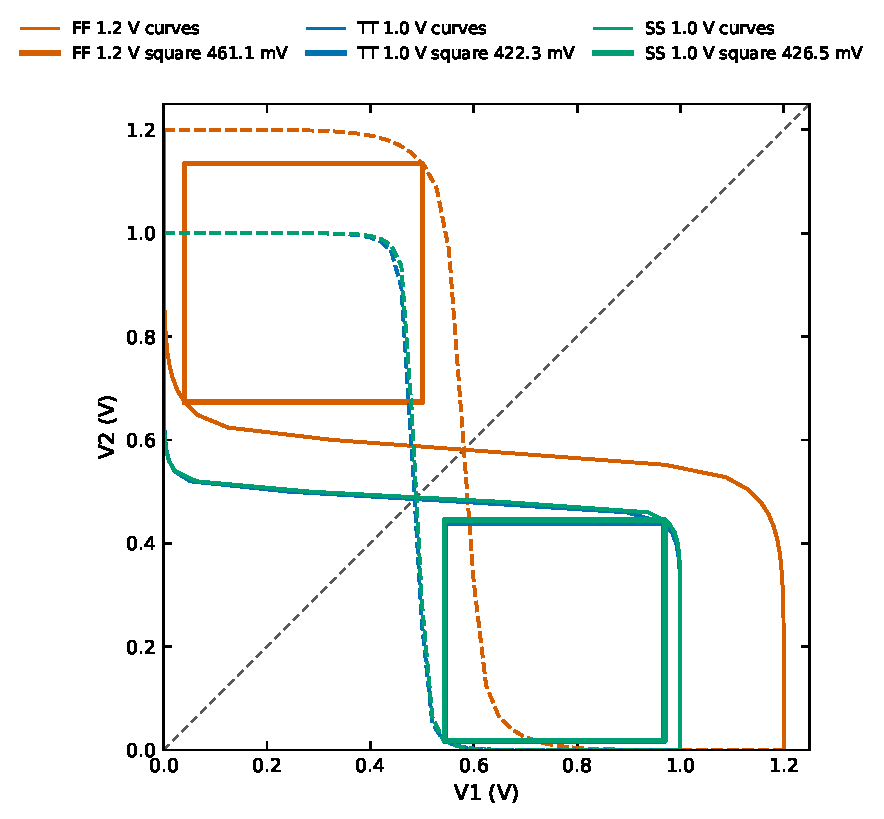
\includegraphics[width=\columnwidth]{figures/baseline_hold_snm_all_corners.pdf}
\caption{Baseline hold-SNM butterfly overlays across corners.}\label{figA:baseline-hold}
\end{figure}

\begin{figure}[h]
\centering
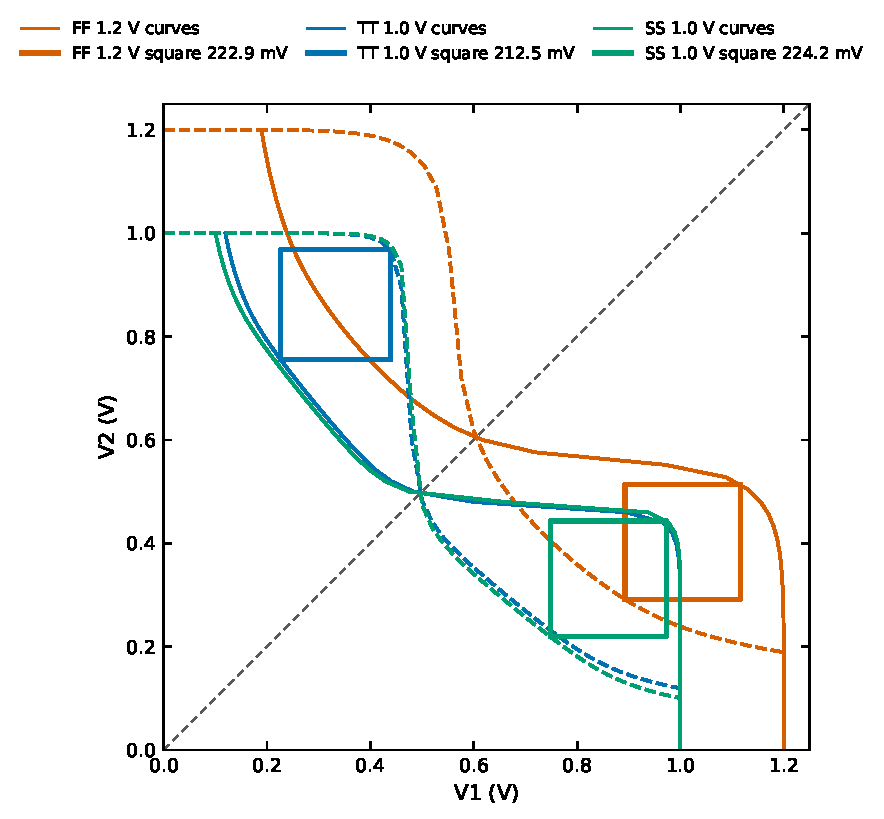
\includegraphics[width=\columnwidth]{figures/baseline_read_snm_all_corners.pdf}
\caption{Baseline read-SNM butterfly overlays across corners.}\label{figA:baseline-read}
\end{figure}

\begin{figure}[h]
\centering
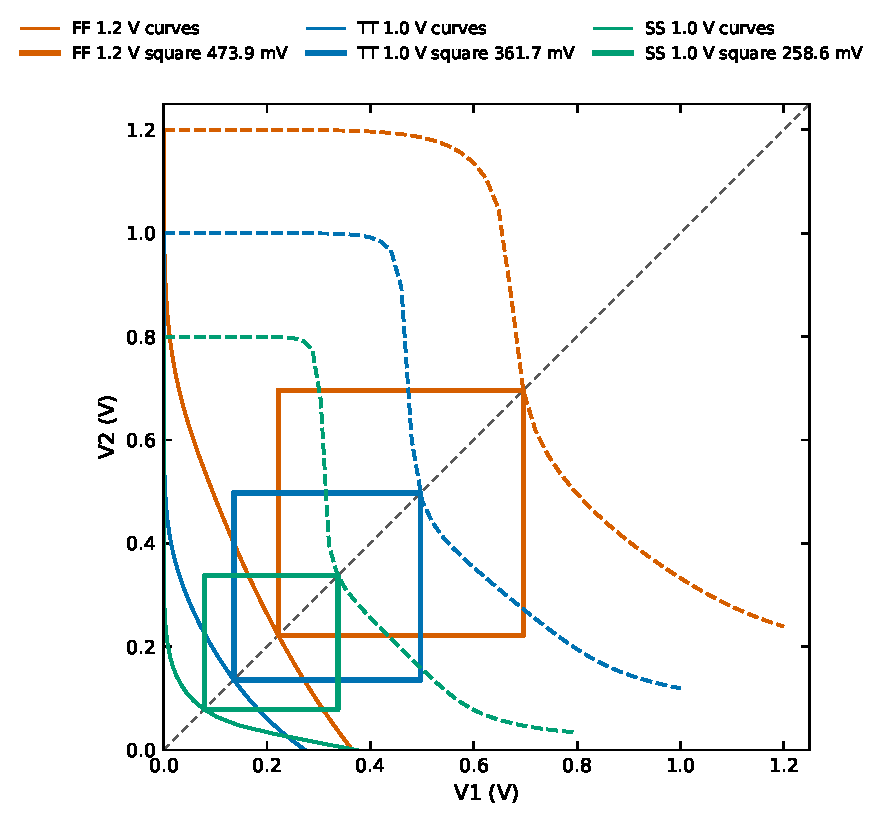
\includegraphics[width=\columnwidth]{figures/baseline_write_nm_all_corners.pdf}
\caption{Baseline WNM butterfly overlays across corners.}\label{figA:baseline-wnm}
\end{figure}

\begin{figure}[h]
\centering
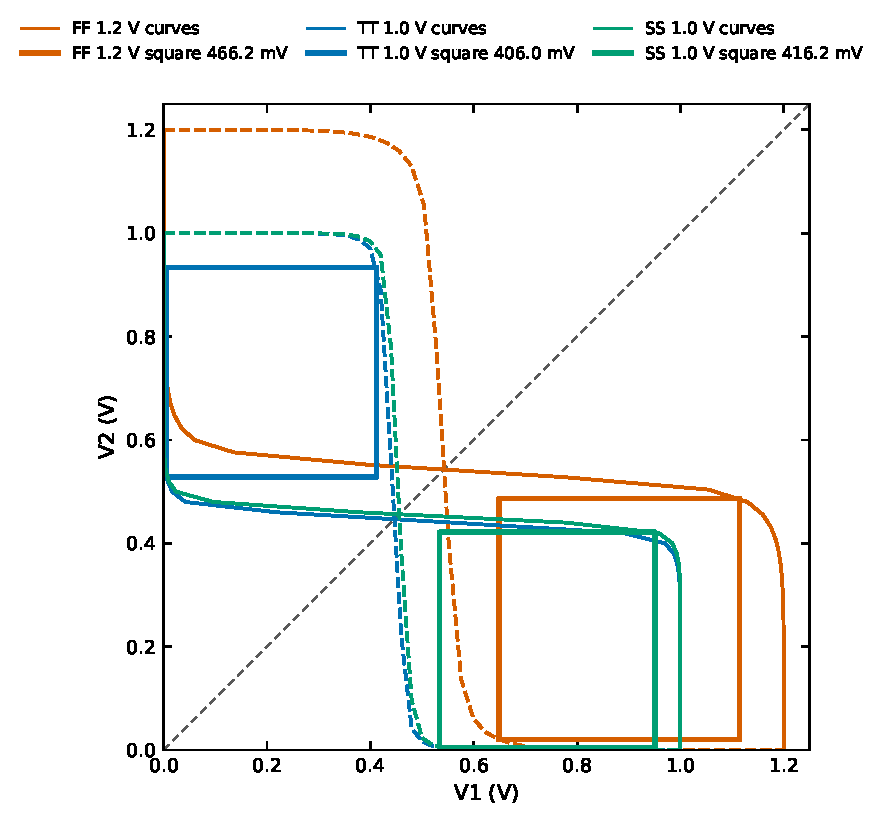
\includegraphics[width=\columnwidth]{figures/high_vt_hold_snm_all_corners.pdf}
\caption{High-$V_t$ hold-SNM butterfly overlays across corners.}\label{figA:hvt-hold}
\end{figure}

\begin{figure}[h]
\centering
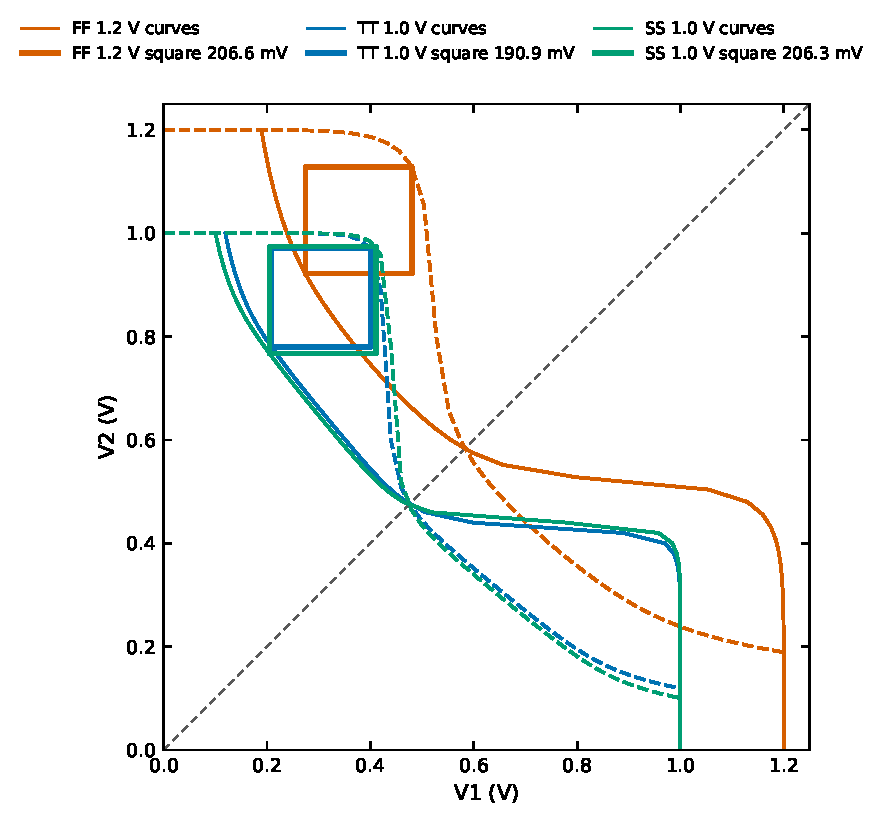
\includegraphics[width=\columnwidth]{figures/high_vt_read_snm_all_corners.pdf}
\caption{High-$V_t$ read-SNM butterfly overlays across corners.}\label{figA:hvt-read}
\end{figure}

\begin{figure}[h]
\centering
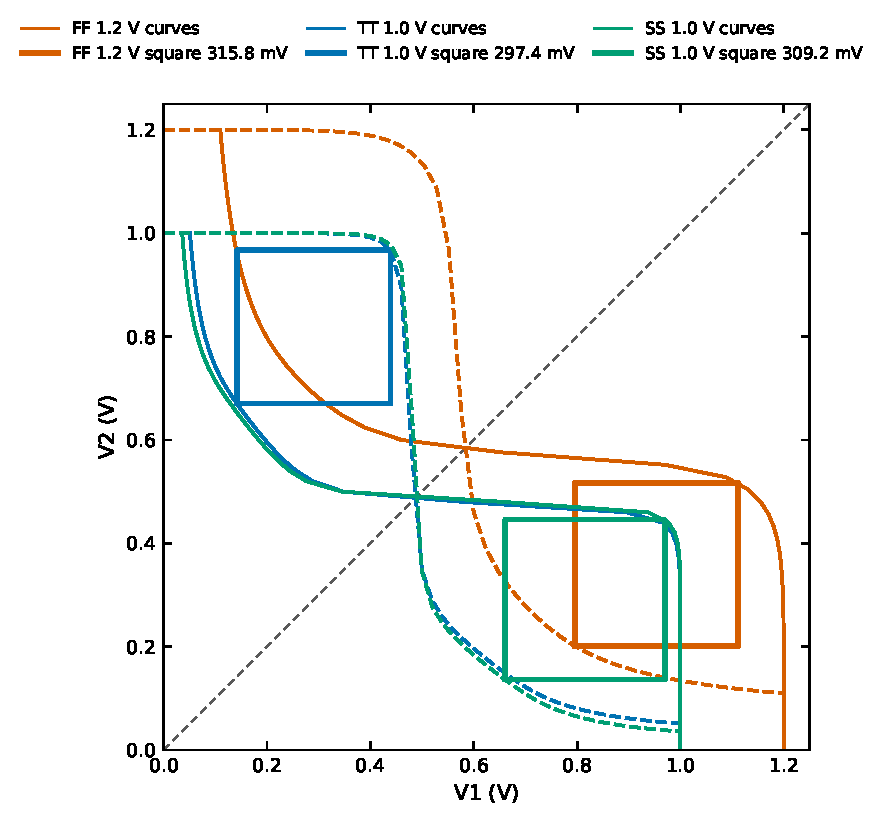
\includegraphics[width=\columnwidth]{figures/wordline_underdrive_read_snm_all_corners.pdf}
\caption{Wordline-underdrive read-SNM butterfly overlays across corners.}\label{figA:wlud-read}
\end{figure}

\section{Negative-BL waveform grid}\label{secB:negbl-waveforms}
\setcounter{figure}{0}
\setcounter{table}{0}

\begin{figure}[h]
\centering
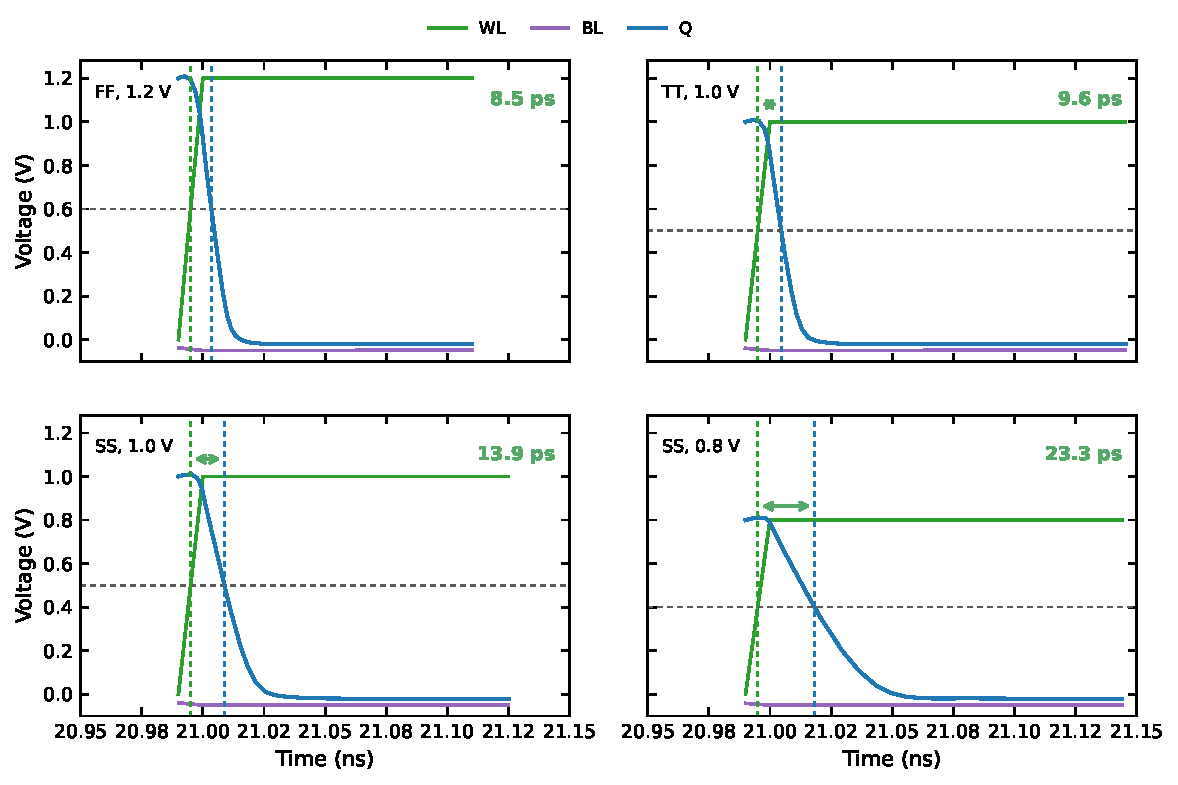
\includegraphics[width=\columnwidth]{figures/negative_bitline_write_delay_grid.pdf}
\caption{Per-corner negative-bitline write-delay waveform grid.}\label{figB:negbl-grid}
\end{figure}

\end{appendices}

\end{document}
